% !TEX root =./main.tex




\begin{abstract}

Sonar, using the data recorded by a phased array of four omni-directional microphones following an omni-directional pulse, allows objects to be detected and imaged.  By calculating the values along a beam (direction), we are able to determine where the object that reflected the sound is located in relation to the sensors.  However, in order to do this, several pre-proessing steps are required.  First, we condition the data: reduce the noise, remove the DC bias, and limit the bandwidth.  Next, we calibrate the data by lining up the recording with the transmission of the pulse and ensuring each channel is recorded evenly.  Next, we compensate for the time-gain by reversing the inverse-square law.  Then, we upsampled by 2.  Finally, we form the beams.  This preprocessing forms the backbone of the sonar system, and is the foundation for the future processing of the beam data into a useable image.


\end{abstract}

\section{Introduction}

This report presents the design process and outcomes for the development of a sonar system by Three Engineers and Ben Corporation. Leveraging advanced digital signal processing (DSP) techniques and MATLAB design tools, our team implemented an 11-stage sonar processing system. Throughout the project, we faced critical engineering decisions to balance the trade-offs between optimizing the system for high-quality sonar imaging and ensuring fast, real-time display capabilities.

The following sections provide a detailed account of our design approach, implementation, and analysis for each stage of the system. By documenting our decisions and their rationale, this report highlights the innovative solutions and technical expertise that distinguish our sonar processing system.

Sonar, ultrasound, and radar are all based on the same principle: transmit a wave, and record its echos.  The only differences are the type of wave or the frequencies involved.  In this project, we are using sonar.  Working in the audible range enables the use of low-cost, common speakers and microphones.  Additionally, it allows us to hear the pulses and echos, which can serve as another problem solving tool.

For this project, we are working with recorded data.  The recorded data was produced using a single omni-directional speaker to transmit the pulse and a phased array of four omni-directional microphones to receive the echos.  Each microphone is given a channel, labeled $X_1$, $X_2$, $X_3$, and $X_4$.

The signal processing is done inside of a \textsc{Matlab} script, following the process diagrammed in Figure \ref{fig:stages}. 

\begin{figure}[H]
    \centering
    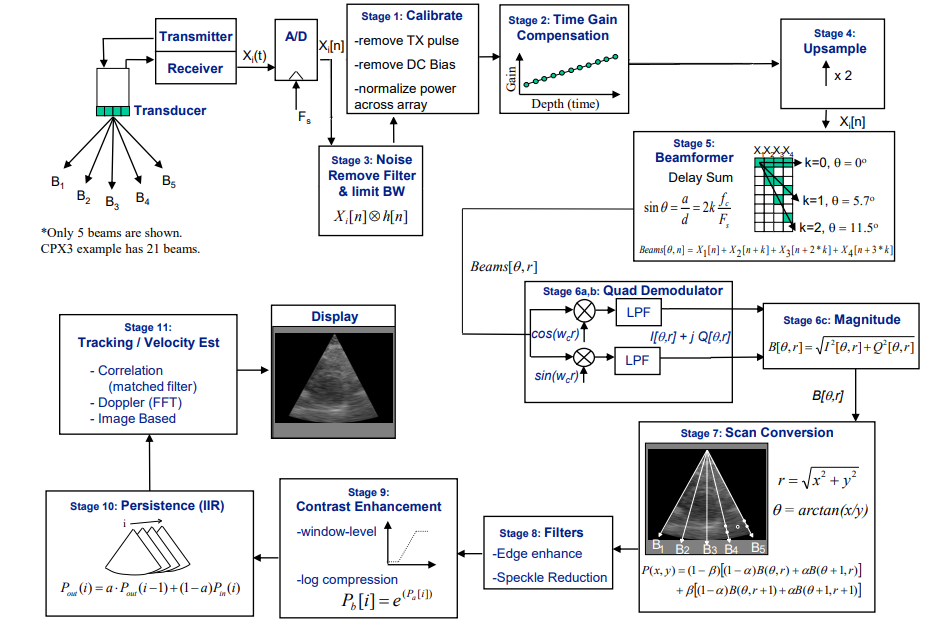
\includegraphics[width=0.75\linewidth]{figures/stages.png}
    \caption{Signal Processing Stages}
    \label{fig:stages}
\end{figure}
